%% use
%% library(cacheSweave)
%% Sweave("unmarked.Rnw", driver = cacheSweaveDriver)


\documentclass[article,shortnames]{jss}
\usepackage{amsmath,amssymb}
\usepackage[utf8]{inputenc}
\usepackage{rotating}
%% need no \usepackage{Sweave.sty}


\DeclareMathOperator{\logit}{logit}
\DeclareMathOperator{\Bern}{Bernoulli}
\DeclareMathOperator{\Bin}{Binomial}
\DeclareMathOperator{\Poi}{Poisson}
\DeclareMathOperator{\MN}{Multinomial}

\newcommand{\um}{\pkg{unmarked}}
\newcommand{\rlang}{\proglang{R}}
\newcommand{\scovs}{\code{siteCovs}}
\newcommand{\ocovs}{\code{obsCovs}}

\author{Ian J. Fiske\\North Carolina State University \And
  Richard Chandler\\ University of Massachusetts Amherst}
\title{\pkg{unmarked}:\\
  An \proglang{R} package for the Analysis of Wildlife Occurrence and Abundance Data}

\Plainauthor{Ian Fiske, Richard Chandler}
\Plaintitle{unmarked: An R Package for the Analysis of Wildlife
  Occurrence and Abundance Data}
\Shorttitle{\um: Analyze Wildlife Data in \proglang{R}}

\Abstract{Ecological research uses data collection techniques that are
  prone to substantial and unique types of measurement error to
  address scientific questions about species abundance and
  distribution.  These data collection schemes include a number of
  site-based methods: occurrence,
  repeated count, distance, removal, double observer sampling.  To
  appropriately analyze these data, two-stage hierarchical
  models have been employed that can separately model explanatory variables of
  both a latent abundance process and a conditional detection process.
  Because these models have a straightforward interpretation
  paralleling how these data arose, they have recently gained immense
  popularity.  The common two-stage structure of these models is
  well-suited for a unified modeling interface.  The \proglang{R}
  package \pkg{unmarked} provides such an unified modeling framework,
  including tools for data exploration, model fitting, model
  criticism, post-hoc analysis, and model comparison.}

\Keywords{ecological, wildlife, hierarchical, occupancy, occurrence, distance, point count}
\Plainkeywords{ecological, wildlife, hierarchical, occupancy, occurrence, distance, point count}


\Address{
Ian Fiske\\
Department of Statistics\\
North Carolina State University\\
2311 Stinson Drive \\
Campus Box 8203 \\
Raleigh, NC 27695-8203 \\
E-mail: \email{ijfiske@ncsu.edu}

Richard Chandler \\   
Department of Natural Resources Conservation \\
University of Massachusetts \\
Room 225 \\
160 Holdsworth Way \\
Amherst, MA 01003-9285 \\
E-mail: \email{rchandler@nrc.umass.edu} 
}



\begin{document}


\section{Introduction}


\subsection{Imperfect detection in ecological research}

One fundamental goal of ecological research is to understand how
environmental variables are related to species abundance or
occurrence.  Addressing these research questions is 
%often challenging because ecologists may face a number of challenges when collecting data on animal prevalence. 
complicated by imperfect detection proability. 
Some animals are difficult to detect because they avoid humans, while others
may have effective camouflage
or simply be so rare that detections are uncommon.  To overcome these
difficulties, ecologists have developed a suite of robust techniques to
sample animal populations.  %A few of these site-based sampling techniques are
These sampling techniques include site occupancy sampling, 
repeated count sampling, transect distance sampling, removal sampling, and 
double observer sampling (see Section~\ref{sec:models-impl-unmark} for 
definitions).  Each of these
sampling methods has some degree of imperfect detection because not
all animals within a visited site are observed.  Observations are
generated by a combination of (1) species abundance and (2) a
detection process that yields observations conditional on the
abundance.  Failure to account for imperfect detection can yield
grossly biased estimates of abundance.  Therefore, the use of these
complex sampling strategies %to collect partially detected data
requires %that the 
statistical models %be used that 
designed to appropriately account for the data collection process.

The scenario described above illustrates how a general unifying data
generation mechanism underlies all of these site-based sampling
techniques.  Specifically, the general statistical model is a
two-level hierarchical model with a \emph{detection} level describing
how the sampling process generates data conditional on latent or
partially observed abundance, density, or occupancy rate, generally
referred to as \emph{state}.  These hierarchical models composed of
(1) state and (2) detection levels will be referred to as two-level
ecological models (TLEMs).  This paper introduces 
\um, an \rlang\ package that provides a unified approach for estimating parameters
for many popular TLEMs.

\subsection[unmarked as a tool for fitting TLEMs]{\pkg{unmarked} as a tool for fitting TLEMs} 

\um\ provides tools to assist researchers %with analyzing data from
%many site-based sampling protocols and fitting TLEMs 
with every step
of the analysis process, including data conversion and exploration, 
visualization, model fitting, post-hoc analysis, and model criticism.  
Because of the
multi-level structure of the data and models, covariate data can exist
at both the state and detection level.  To succinctly describe these
data, \um\ uses a new data type called the \code{unmarkedFrame}
(Section~\ref{sec:data-requirements}).  
\um\ provides functions that
import data from various common formats and convert it into \um's data
types.  Once imported, \um\
provides functions to summarize and subset these data in a manner
familiar to users of \rlang's more common data structures such as
vectors, matrices, and data frames. \um\ provides model-fitting
functions for each of the TLEMs.  The fitting functions each find the
maximum likelihood estimates of parameters from a particular TLEM
(Section~\ref{sec:fitting-models}) and return an object that can be 
%queried for a variety of common post-hoc analyses % analysis -> analyses
easily manipulated. Methods exist for performing numerous post-hoc analyses
such as requesting linear combinations of parameters, 
back-transforming parameters to constrained scales,
determining confidence intervals, and evaluating goodness of fit.  The model
specification syntax of the fitting functions was designed in such a
way that it is quite familiar to users of \rlang's common fitting
functions such as \code{lm} for fitting linear models.

Although there is existing software for fitting some TLEMs
\citep[e.g.,][for occupancy models]{Hines2002}, there are a number of
advantages to a unified TLEM-fitting framework within \rlang.  Many
researchers are already familiar with \rlang\ and use its powerful
data manipulation and plotting capabilities.  
% to clean and explore their data.
Sometimes many
species are analyzed in tandem, so that a common method of aggregating
and post-processing of results is needed, a task easily accomplished
in \rlang.  All of this is made much simpler by analyzing the data
%using 
within \rlang, and using a single environment to complete all phases of 
the analysis is much less error-prone than switching between applications.
% the researcher to avoid switching
%applications.  After all, each time the data go through some
%processing step or translation between applications, additional
%programming is required, introducing more opportunities for hidden
%data errors.  
Another important advantage of \um's approach is
that researchers can easily simulate and analyze data within the same
computational environment.  This work flow permits the computation of
power analyses or designing for planning sampling plans.  An
alternative approach for fitting TLEMs is for researchers to program
their own likelihood and maximize it.  However, this requires that the
researcher have well-developed programming abilities and also can
require significant amount of overhead replicating code with minor
tweaks for each new set of data.  \um\ provides a sufficiently
flexible framework that many proposed models may be fit without
extensive programming by the applied researcher.

In this paper, Section~\ref{sec:models-impl-unmark} %first 
gives a brief % give -> gives
summary of many of the models \um\ is capable of fitting.  %Then,
Section~\ref{sec:unmarked-usage} %will 
describes general \um\ usage %describe -> describes
accompanied by a running data example to illustrate the usage.

\section[Models implemented in unmarked]{Models implemented in \um}
\label{sec:models-impl-unmark}

\pkg{unmarked} finds maximum likelihood estimates for the parameters
of many TLEMs for %many 
popular types of site-based sampling protocols.
This section provides a summary of several of these sampling
techniques and how TLEMs can be used to model the resulting data.
This section also introduces the syntax to illustrate how nicely it
parallels the model structure, but full usage %will be 
is described in
Section~\ref{sec:unmarked-usage}.


\begin{sidewaystable} \small
\begin{tabular}{c|ccc}
\textbf{Model} & \textbf{Fitting function} & \textbf{Data} & \textbf{Citation} \\ \hline
Occupancy & \code{occu} & unmarkedFrameOccu & \citep{MacKenzie2002} \\
Royle-Nichols & \code{occuRN}& unmarkedFrameOccu & \citep{Royle2003} \\
Point Count &\code{pcount}& unmarkedFramePCount & \citep{Royle2004} \\
Distance-sampling &\code{distsamp}& unmarkedFrameDS & \citep{Royle2004b} \\
Arbitrary multinomial-Poisson &\code{multinomPois}& unmarkedFrameMPois & \citep{Royle2004a} \\
Colonization-extinction &\code{colext}& unmarkedMultFrame & \citep{MacKenzie2003}
\end{tabular}
\caption{Models handled by unmarked along with their associated
  fitting function (Section~\ref{sec:models-impl-unmark}) and data
  type (Section~\ref{sec:data-requirements}).}
\label{tab:models}
\end{sidewaystable}


\subsection{Occurrence data} 
\label{sec:occ}

A popular estimand of interest in ecological research is the
proportion of sites that are used by the study species, called
occupancy rate.  Another related goal is to identify factors that are
associated with the changes in the probability of a site being
occupied.  To estimate these parameters, researchers can employ
so-called occurrence sampling, whereby surveyors visit a sample of $M$
sites and record the binary response of species detection (1) or
non-detection (0) during $J_{i}$ visits to the $i$th site during a
`season' \citep{MacKenzie2002}.  The key assumptions that are made
when modelling these data are that the occupancy state at a site is
assumed to remain constant throughout the season and repeated visits at
a site are independent.

The repeated visits are necessary to gain information about the
detection rate separate from the occupancy rate.  To describe these
data, we use the following hierarchical Bernoulli.  Let $\psi_i$ be
the probability of occupancy at site $i$.  And $p_{ij}$ is the
probability of detecting the species at site $i$ during the $j$th
observation given that site $i$ is truly occupied.  More formally,
observations at site $i$ arise as
\begin{gather}
Z_i \sim \Bern(\psi_i) \\
Y_{ij}|Z_i \sim \Bern(Z_i p_{ij})\text{\quad for $j=1,2,\dots,J_{i}$},
\end{gather}
where $Z_i$ is the partially observed occupancy state.

Variables that are suspected to be related to the occupancy state are
modeled as
\begin{gather}
  \logit(\psi_i) = \mathbf x_i' \mathbf \beta,
\end{gather}
where $\mathbf x_i$ is a $p$-vector of site-level covariates and $\mathbf \beta$
is a $p$-vector of their corresponding effect parameters.  Similarly, the
probability of detection can be modeled with
\begin{gather}
  \logit(p_{ij}) = \mathbf v_{ij}' \mathbf \alpha,
\end{gather}
where $\mathbf v_{ij}$ is a $q$-vector of observation-level covariates and
$\mathbf \alpha$ is a $q$-vector of their corresponding effect parameters.

\subsubsection[Fitting occupancy models in unmarked]{Fitting occupancy models in \um}

The above occupancy model can be fit in \um\ using the \code{occu}
fitting function.
\begin{Code}
  occu(formula, data, knownOcc, starts, method, control, se)
\end{Code}
where 
\begin{itemize}
\item \code{formula} is formula that specifies the covariates of
  detection and state in the double right-hand-sided formula: \code{~
    v.1 + ... + v.k ~ x.1 + ... + x.l }.  Standard \rlang\ syntax for
  interactions and other formula modifications such as offsets and
  arbitrary functions are available.  Categorical variables can be
  include by simply specifying factors in the formula.
\item \code{data} is the input data as an
  \code{unmarkedFrameOccu} object.
\item \code{knownOcc} is a numeric vector providing the indices of
  any sites that were known to be occupied during the sampling.
  These sites are sometimes included to provide extra information
  about the detection parameters only.
\item \code{starts} allows the user to optionally supply starting
  values to the optimizer.
\item \code{method} and \code{control} are directly fed into
  \rlang's \code{optim} function, which provides the optimization
  engine.  They allow fine control of the optimization algorithm.
  The default settings are to use the quasi-Newton Broyden,
  Fletcher, Goldfarb and Shanno (BFGS) algorithm.
\item \code{se} is a Boolean that specifies whether or not to
  return a standard error computed from the Hessian.
\end{itemize}



\subsection{Repeated count data}
\label{sec:repeated-count-data}

Estimates of occupancy rate provide much less information about a
population than do abundance estimates. For instance, suppose the
average number of individuals per site decreases from 10 to 5 during
the course of a multi-season study. This dramatic population decline
would not be detected using occurence sampling.  One method to
estimate abundance is to repeatedly visit a sample of $M$ sites and
record the number of unique individuals observed at each site.
Similar assumptions are made as with occurrence data: (1) abundance at
a site remains constant during a season and (2) counts at a site are
independent.  \citet{Royle2004} presented the following TLEM for
repeated count data.  Let $N_i$ is the unobserved total number of
animals using a site and $Y_{ij}$ is the number of animals observed
during the $j$th visit.  Then,
\begin{gather}
  N_i \sim F(\lambda_i, \theta) \label{eq:pc2} \\
  Y_{ij}|N_{i} \sim \Bin(N_i, p_{ij})\text{\quad for $j=1,2,\dots,J_{i}$},
\end{gather}
where $\lambda_i$ is the abundance rate at site $i$ and $p_{ij}$ is
the detection probability during the $j$th visit to site $i$.  $F$ is
a discrete distribution with support restricted to $N_{i} \ge 0$ and
$\theta$ are extra parameters of $F$ other than the location
parameter, $\lambda_{i}$.  \um\ currently supports $F$ as Poisson or
negative binomial.  In the Poisson case, there is no $\theta$.  In the
negative binomial case, $\theta$ is a dispersion parameter, which is
useful when overdispersion is suspected.

As with the occupancy TLEM, covariates may be included in either the
state (here, abundance) or detection levels, but abundance is modeled
through a log link to enforce it's positivity constraint.
\begin{gather}
  \log(\lambda_i) = \mathbf x_i' \mathbf \beta,
\end{gather}
where $\mathbf x_i$ is a $p$-vector of site-level covariates and $\mathbf \beta$
is a $p$-vector of their corresponding effect parameters.  Similarly, the
probability of detection can be modeled with
\begin{gather}
  \logit(p_{ij}) = \mathbf v_{ij}' \mathbf \alpha,
\end{gather}
where $\mathbf v_{ij}$ is a $q$-vector of observation-level covariates and
$\mathbf \alpha$ is a $q$-vector of their corresponding effect parameters.

\subsubsection[Fitting repeated count models in unmarked]{Fitting repeated count models in \um}

The \um\ fitting function \code{pcount} estimates parameters in a
\eqref{eq:pc2}.

\begin{Code}
pcount(formula, data, K, mixture, starts, method, control, se)
\end{Code}
where 
\begin{itemize}
\item \code{formula} is formula that specifies the covariates of
  detection and state in the double right-hand-sided formula: \code{~
    v.1 + ... + v.k ~ x.1 + ... + x.l }.  Standard \rlang\ syntax for
  interactions and other formula modifications such as offsets and
  arbitrary functions are available.  Categorical variables can be
  include by simply specifying factors in the formula.
\item \code{data} is the input data as an
  \code{unmarkedFramePCount} object.
\item \code{K} is the upper index if summation used to integrate out
  $N_{i}$ in to compute the likelihood in Equation~\eqref{eq:pc2}.
\item \code{mixture} specifies whether $F$ is Poisson or negative
  binomial, taking values \code{``P''} or \code{``NB''} respectively.
\item see Section~\ref{sec:occ} for details on the \code{starts},
  \code{method}, and \code{se} arguments.
\end{itemize}

     
\subsection{General multinomial-Poisson TLEM}

Here we discuss a more general TLEM that can be modified to fit a
variety of ecological sampling methods, the multinomial-Poisson model
\citep{Royle2004a}.  The general form of this model is
\begin{gather}
  N_i \sim \Poi(\lambda_i) \label{eq:mp2} \\
  \mathbf Y_i|N_{i} \sim \MN(N_i, \boldsymbol \pi_i),
\end{gather}
where $N_i$ is the latent abundance at site $i$ as with the point
count model, and $\boldsymbol \pi_i=(\pi_{i1},\pi_{i2},\pi_{iJ})'$ is
the vector of cell probabilities of observing responses in the $J$
possible categories, and $\mathbf Y_{i}$ is the $J$-vector of counts
that were actually observed.  In general, $\boldsymbol \pi_i$ is
determined by the specific sampling method and
$\sum_{j} \pi_{ij} \le 1$ because detection is imperfect and
$1 - \sum_{j} \pi_{ij} \le 1$ is the probability of the species
escaping detection at site $i$.  

For multinomial-Poisson sampling methods, the actual observations are
an underlying categorical detection variable with $R \leq J$ levels so
that the $J$-dimensional $\mathbf Y_{i}$ is derived from the
$R$-dimensional raw counts in some sampling method-specific manner.
Thus, it is necessary to model the detection at the raw observation
level, denoted $p_{ik}$ for $k=1,2,\dots,R$ at site $i$.  Then we
derive the multinomial cell probabilities $\boldsymbol \pi_{i}$
through the sampling technique-specific relationship
$\pi_{ij}=g(p_{ik})$ where $p_{ik}$ is the underlying probability of
detection and $g$ is some sampling method-specific function.  

Thus,
the only two requirements to adapt \um's general multinomial Poisson
modeling to a new sampling method is to specify $g$ and a binary 0-1
matrix that describes the mapping of elements of
$\mathbf p_{i} = (p_{i1},\dots,p_{iR})'$ to elements of
$\boldsymbol \pi_{i}$.  This mapping matrix, referred to in
\um\ as \code{obsToY}, is necessary to consistently clean
missing values from the data and relate observation-level covariates
with the responses.  The ($j$,$k$)th element of
\code{obsToY} is 1 only if $p_{ik}$ is involved in the computation of
$\pi_{ij}$.  The detection function $g$ is called \code{piFun} in \um.

Covariates may be included in either the
state (here, abundance) or detection levels, through $\mathbf p_{i}$
(not $\boldsymbol \pi_{i}$).
\begin{gather}
  \log(\lambda_i) = \mathbf x_i' \mathbf \beta,
\end{gather}
where $\mathbf x_i$ is a $p$-vector of site-level covariates and $\mathbf \beta$
is a $p$-vector of their corresponding effect parameters.  Similarly, the
probability of detection can be modeled with
\begin{gather}
  \logit(p_{ij}) = \mathbf v_{ij}' \mathbf \alpha,
\end{gather}
where $\mathbf v_{ij}$ is a $q$-vector of observation-level covariates and
$\mathbf \alpha$ is a $q$-vector of their corresponding effect parameters.

\subsubsection[Fitting multninomial-Poisson models in unmarked]{Fitting multinomial-Poisson models in \um}
  
The \code{multinomPois} fitting function is available in \um\ for
fitting multinomial-Poisson TLEMs.

\begin{Code}
multinomPois(formula, data, starts, method, control, se)
\end{Code}
where 
\begin{itemize}
\item \code{formula} is formula that specifies the covariates of
  detection and state in the double right-hand-sided formula: \code{~
    v.1 + ... + v.k ~ x.1 + ... + x.l }.  Standard \rlang\ syntax for
  interactions and other formula modifications such as offsets and
  arbitrary functions are available.  Categorical variables can be
  include by simply specifying factors in the formula.
\item \code{data} is the input data as an
  \code{unmarkedFrameMPois} object.
\item see Section~\ref{sec:occ} for details on the \code{starts},
  \code{method}, and \code{se} arguments.
\end{itemize}

We now describe two common sampling methods that can be modeled
with the multinomial-Poisson model: removal sampling and double
observer sampling.  These two methods are included in \um, but
additional methods may easily be specified by the user with only the
\code{piFun} function and \code{obsToY} matrix.

\subsubsection{Removal sampling}

Popular in fisheries, removal sampling is implemented by visiting a
sample of $M$ sites $J$ times each and trapping and removing
individuals at each visit with the same effort.  Thus, $Y_{ij}$ is the
number of individuals captured at the $j$th visit for $j=1,2,\dots,J$.

Then, we can specify $g$ for removal sampling as follows.  The
probability of an individual at site $i$ being captured on the first
visit is $\pi_{i1} = p_{i1}$.  The probability of capture on the $j$th
visit is
\begin{equation}
  \pi_{ij} = \prod_{k=1}^{j-1}(1 - p_{ik})p_{ij},
\end{equation}
for $j=2,\dots,J$ and the probability of not being sampled is
\begin{equation}
  \pi_{i,J+1} = \prod_{j=1}^{J}(1-p_{ij})
\end{equation}
Or, equivalently,
\begin{equation}
  \mathbf \pi_i =
  \begin{pmatrix}
    p_{i1} \\
    (1-p_{i1})p_{i2} \\
    \vdots \\
    \prod_{j=1}^J(1-p_{ij})p_{iJ}
  \end{pmatrix}
\end{equation}
Thus, the mapping matrix is an $J \times R$ upper triangular matrix with ones in
the upper triangle,
\begin{equation}
  \begin{pmatrix}
    1 & 1 & \dots & 1 \\
    0 & 1 & \dots & 1 \\
    \vdots & & \ddots & \vdots \\
    0 & 0 & \dots  & 1
  \end{pmatrix}
\end{equation}


\subsubsection{Double observer sampling}
\label{sec:double-observ-sampl}

Double observer sampling collects data by a team of two surveyors
simultaneously visiting a site.  They each collect lists of identified
animals.  Thus the counts in the three cells of $\mathbf Y_i$
correspond to the numbers of individuals seen by observer one,
observer two, or both.  Thus, for double observer sampling, $g$ is
defined as follows.
\begin{equation}
  \mathbf \pi_i =
  \begin{pmatrix}
    p_{i1}(1-p_{i2}) \\
    (1-p_{i1})p_{i2} \\
    p_{i1}p_{i2} \\
    (1-p_{i1})(1-p_{i2}).
  \end{pmatrix}
\end{equation}
The \code{obsToY} mapping matrix for double observer sampling is the
following $3 \times 2$ matrix.
\begin{equation}
  \begin{pmatrix}
    1 & 0 \\
    0 & 1 \\
    1 & 1 
  \end{pmatrix}
\end{equation}

\subsection{Distance sampling}

In distance sampling, surveyors sample sites by traveling along a
transect or standing at a so-called point transect and recording the
distance to each detected study animal
\citep{Thomas2010}.  For the model of \citep{Royle2004b} used in \um\,
the continuous distances to each observed animal must be binned into 
categories according to cut-points $c_1, c_2,\dots,c_{J}$.  
Then  $Y_{ij}$ is the count of observations at site $i$ falling into
the $j$th distance bin.  The user must specify a
detection function $g(x;\theta)$ that describes the probability of
observing an animal as a function of distance $x$ from the transect. 
The cell probabilities $\mathbf \pi_i$ are
constructed by integrating $g$ over the distance classes.

As currently implemented, the general form of the distance sampling model
is identical to the multinomial-Poisson mixture described above, with the
sole difference being that instead of
\begin{gather}
  \logit(p_{ij}) = \mathbf v_{ij}' \mathbf \alpha,
\end{gather}
we have 
\begin{gather}
  \log(\theta_i) = \mathbf v_{i}' \mathbf \alpha,
\end{gather}
Here, the log link is required because $\theta$ is a positive shape parameter 
of the detection function. Eventually, alternative models of the latent 
abundance variable (\emph{eg}, the negative binomial) may be added.


\subsubsection[Fitting distance sampling models in unmarked]{Fitting distance sampling models in \pkg{unmarked}}

The above distance model can be fit in \um\ using the \code{distsamp}
fitting function.

\begin{Code}
distamp(formula, data, keyfun = c("halfnorm", "exp", "hazard", 
    "uniform"), output = c("density", "abund"), unitsOut = c("ha", 
    "kmsq"), starts = NULL, method = "BFGS", control = list(), 
    se = TRUE)
\end{Code}

\begin{itemize}
    \item \code{formula} is formula that specifies the covariates of
        detection and state in the double right-hand-sided formula: \code{~
        v.1 + ... + v.k ~ x.1 + ... + x.l }.  Standard \rlang\ syntax for
        interactions and other formula modifications such as offsets and
        arbitrary functions are available.  Categorical variables can be
        include by simply specifying factors in the formula.
    \item \code{data} is the input data as an
        \code{unmarkedFrameDS} object.
    \item \code{keyfun} specifies the detection function.
    \item \code{output} determines how the response is modeled when all
        transect lengths and distance intervals are equal. Otherwise, 
        the matrix of site by distance interval areas must be accounted for
        and density is modeled.
    \item \code{unitsOut} the output units when modeling density.
    \item see Section~\ref{sec:occ} for details on the \code{starts},
      \code{method}, and \code{se} arguments.
  \end{itemize}
  
  \subsection{Colonization-extinction data}

Sometimes the study objective is to understand the evolution of
occupancy state over time.  To obtain such information %about change in the
%occupancy state variable over time, surveyors 
researchers conduct repeated occupancy
studies (see Section~\ref{sec:occ}) to the same sample of sites over
consecutive seasons \citep{MacKenzie2003}.  They then seek to estimate
probabilities of colonization ($\gamma_{it}$) and extinction
($\epsilon_{it}$), where colonization is the change of an unoccupied
site to occupied and extinction if the change of an occupied site to
unoccupied.  If the occupancy status is assumed to evolve according to
a Markov process, then a 2-state finite hidden Markov model describes
these data.  Let $Y_{itj}$ denote the observed animal occurrence
status at visit $j$ during season $t$ to site $i$.  Then
\begin{gather}
  Z_{i1} \sim \Bern(\psi) \\
  Z_{it} \sim
  \begin{cases}
    \Bern(\gamma_{i(t-1)}) & \text{if $Z_{i(t-1)} = 0$} \\
    \Bern(1-\epsilon_{i(t-1)}) & \text{if $Z_{i(t-1)} = 1$}
  \end{cases}, \\
  \text{for $t=2,3,\dots,T$} \notag \\
  Y_{itj} | Z_{it} \sim \Bern(Z_{it} p_{itj})
\end{gather}

\subsubsection[Fitting colonization-extinction models in
unmarked]{Fitting colonization-extinction models in \um}

Colonization-extinction models in \um\ are fit with the \code{colext}
fitting function.

\begin{Code}
  colext(psiformula, gammaformula, epsilonformula, pformula, data, 
  starts, method, control, se)
\end{Code}
       
\begin{itemize}
\item \code{psiformula} is a right-hand sided formula for the initial probability of
  occupancy ($\psi$) at each site.
\item \code{gammaformula} is a right-hand sided formula for
  colonization probability ($\gamma$).
\item \code{epsilonformula} is a right-hand sided formula for
  extinction probability ($\epsilon$).
\item \code{pformula} is a right-hand sided formula for detection probability.
\item \code{data} is an unmarkedMultFrame object that supplies the data.
\item see Section~\ref{sec:occ} for details on the \code{starts},
  \code{method}, and \code{se} arguments.
\end{itemize}

\section[unmarked usage]{\pkg{unmarked} usage}
\label{sec:unmarked-usage}

By exploiting the common structure of TLEMs, \um\ is able to
provide data structures, fitting syntax, and post-processing that form
a cohesive framework for site-based ecological data analysis.  In
order to achieve these goals, \um\ uses the S4 class system
\citep{Chambers2008}. As \rlang's most modern system of class-based
programming,  S4 allows 
%re-use of common function names (called methods) for different data types as arguments.  
customization of functions, referred to as methods, to specific object classes and 
superclasses. For example, when
\code{predict}, a common
method, is called with any \um\  model fit
object as an argument, the actual \code{predict} implementation depends on the
specific TLEM that was fit.  Use of class-based programming can provide
more reliable and maintainable software while also making the program
more user-friendly \citep{Chambers2008}.


\subsection{Preparing data}
\label{sec:data-requirements}

\um\ uses a custom S4 data structure called the unmarkedFrame
to store all data related to a sampling survey.  Although this at
first appears to add an extra layer of work for the user, there are
several reasons for this design choice.  The multilevel structure of
TLEMs means that standard rectangular data structures such as data
frames or matrices are not suitable for storing the data.  For
example, covariates might have been measured separately at the site
level and at the visit level.  Furthermore, the length of the response
vector $\mathbf Y_{i}$ at site $i$ might differ from the number of
observations at the site as in the multinomial Poisson model.  Aside
from these technical reasons, \citet{Gentleman2009} pointed out that
the use of such portable custom data objects can simplify future
reference to previous analyses, an often neglected aspect of research.
Repeated fitting calls using the same set of data require less code
repetition if all data is contained in a single object.  Finally,
calls to fitting functions have a cleaner appearance with a more
obvious purpose when the call is not buried in data arguments.  The
parent data class is called an unmarkedFrame and each \um\
fitting function has its own data type that extends the
unmarkedFrame.  Thus, the first step when using \um\ is to
import data into the proper type of unmarkedFrame.  To ease
this step, \um\ includes several helper functions to automatically
convert data into an unmarkedFrame: \code{csvToUMF} which
imports data directly from a comma-separated value text file,
\code{formatWide} and \code{formatLong} which convert data from data
frames, and the family of unmarkedFrame constructor functions.

An unmarkedFrame object contains slots for the observation matrix
\code{y}, a data frame of site-level covariates \code{siteCovs}, and a
data frame of observation-level covariates \code{obsCovs}.  The
\code{y} matrix is the only required unmarkedFrame slot.  \code{y} is
an $M \times J$ matrix with the $i$th row containing the
$J$-dimensional $\mathbf y_i$.  If $J_{i} \le J$, then any number of
elements of $\mathbf y_{i}$ can take the value \code{NA} to denote
this.  \code{siteCovs} is an $M$-row data frame with a column for each
site-level covariate.  \code{obsCovs} is an $MJ$-row data frame with a
column for each observation-level covariate.  Thus each row of
\code{obsCovs} corresponds to a particular observation, with the order
corresponding to site varying slower and observation within site
varying faster.  Both \scovs\ and \ocovs\ can contain \code{NA}
values corresponding to unbalanced data collection.  If any terms in the model
specification are missing for that observation, \um\
automatically removes observations.  \um\ provides
constructor functions to make creating unmarkedFrames straightforward.
For each specific data type, specific types of unmarkedFrames extend
the basic unmarkedFrame to handle model-specific nuances.

Here is an example of creating an unmarkedFrame for point count data
from a list a matrix of observations, a data frame of site-level
covariates, and a list of matrices of observation-level covariates.
\pkg{unmarked} seamlessly displays the unmarkedFramePCount object as a
data frame.

First, load the included data set of avian point counts from
\citet{Kery2005} and visually inspect the point count matrix, which is
already in the same format as the \code{y} slot of an unmarkedFrame.

\begin{Schunk}
\begin{Sinput}
> library(unmarked)
> data(mallard)
> head(mallard.y)
\end{Sinput}
\begin{Soutput}
     y.1 y.2 y.3
[1,]   0   0   0
[2,]   0   0   0
[3,]   3   2   1
[4,]   0   0   0
[5,]   3   0   3
[6,]   0   0   0
\end{Soutput}
\begin{Sinput}
> dim(mallard.y)
\end{Sinput}
\begin{Soutput}
[1] 239   3
\end{Soutput}
\end{Schunk}

So the data have 239 sites and a maximum of
3 observations per site. 
  
In this example, site-level covariates are already in the same data
frame format as the \scovs\ slot.  

\begin{Schunk}
\begin{Sinput}
> summary(mallard.site)
\end{Sinput}
\begin{Soutput}
      elev                length               forest          
 Min.   :-1.436e+00   Min.   :-4.945e+00   Min.   :-1.265e+00  
 1st Qu.:-9.565e-01   1st Qu.:-5.630e-01   1st Qu.:-9.560e-01  
 Median :-1.980e-01   Median : 4.500e-02   Median :-6.500e-02  
 Mean   :-4.603e-05   Mean   :-2.929e-05   Mean   : 6.695e-05  
 3rd Qu.: 9.940e-01   3rd Qu.: 6.260e-01   3rd Qu.: 7.900e-01  
 Max.   : 2.434e+00   Max.   : 2.255e+00   Max.   : 2.299e+00  
\end{Soutput}
\end{Schunk}


However observation level covariates
are a list object with separate $M \times J$ matrices for each
observation-level covariate.  The unmarkedFrame constructors can
accept \ocovs\ in this list format or as a data frame in the format
described above.

\begin{Schunk}
\begin{Sinput}
> str(mallard.obs)
\end{Sinput}
\begin{Soutput}
List of 2
 $ ivel: num [1:239, 1:3] -0.506 -0.934 -1.136 -0.819 0.638 ...
  ..- attr(*, "dimnames")=List of 2
  .. ..$ : NULL
  .. ..$ : chr [1:3] "ivel.1" "ivel.2" "ivel.3"
 $ date: num [1:239, 1:3] -1.76 -2.9 -1.69 -2.19 -1.83 ...
  ..- attr(*, "dimnames")=List of 2
  .. ..$ : NULL
  .. ..$ : chr [1:3] "date.1" "date.2" "date.3"
\end{Soutput}
\end{Schunk}

The following call to \code{unmarkedFramePCount} function creates an
unmarkedFramePCount object, which is the specific type of
unmarkedFrame for point count data.

\begin{Schunk}
\begin{Sinput}
> mallardUMF <- unmarkedFramePCount(y = mallard.y, siteCovs = mallard.site, 
+     obsCovs = mallard.obs)
\end{Sinput}
\end{Schunk}

Printing unmarkedFrames shows them as data frames to make it easier to
verify that the data was converted correctly.

\begin{Schunk}
\begin{Sinput}
> head(mallardUMF)
\end{Sinput}
\begin{Soutput}
Data frame representation of unmarkedFrame object.
   y.1 y.2 y.3   elev length forest ivel.1 ivel.2 ivel.3 date.1 date.2 date.3
1    0   0   0 -1.173  0.801 -1.156 -0.506 -0.506 -0.506 -1.761  0.310  1.381
2    0   0   0 -1.127  0.115 -0.501 -0.934 -0.991 -1.162 -2.904 -1.047  0.596
3    3   2   1 -0.198 -0.479 -0.101 -1.136 -1.339 -1.610 -1.690 -0.476  1.453
4    0   0   0 -0.105  0.315  0.008 -0.819 -0.927 -1.197 -2.190 -0.690  1.239
5    3   0   3 -1.034 -1.102 -1.193  0.638  0.880  1.042 -1.833  0.167  1.381
6    0   0   0 -0.848  0.741  0.917 -1.329 -1.042 -0.899 -2.619  0.167  1.381
7    0   0   0 -0.910  0.115 -1.083 -1.448 -1.562 -1.676 -2.690 -1.190  1.596
8    0   0   0 -1.003 -1.007 -0.792 -0.321 -0.557 -0.636 -2.119 -0.476  1.453
9    0   0   0 -0.058 -0.913  0.553 -0.231 -0.231 -0.001 -2.047 -0.547  1.167
10   0   0   0 -0.631  1.556  0.808 -1.097 -1.021 -0.832 -2.333 -1.119 -0.261
\end{Soutput}
\end{Schunk}

We can also check data contents with a quick summary.

\begin{Schunk}
\begin{Sinput}
> summary(mallardUMF)
\end{Sinput}
\begin{Soutput}
unmarkedFrame Object

239 sites
Maximum number of observations per site: 3 
Mean number of observations per site: 2.76 
Sites with at least one detection: 40 

Tabulation of y observations:
   0    1    2    3    4    7   10   12 <NA> 
 576   54   11    9    6    1    1    1   58 

Site-level covariates:
      elev                length               forest          
 Min.   :-1.436e+00   Min.   :-4.945e+00   Min.   :-1.265e+00  
 1st Qu.:-9.565e-01   1st Qu.:-5.630e-01   1st Qu.:-9.560e-01  
 Median :-1.980e-01   Median : 4.500e-02   Median :-6.500e-02  
 Mean   :-4.603e-05   Mean   :-2.929e-05   Mean   : 6.695e-05  
 3rd Qu.: 9.940e-01   3rd Qu.: 6.260e-01   3rd Qu.: 7.900e-01  
 Max.   : 2.434e+00   Max.   : 2.255e+00   Max.   : 2.299e+00  

Observation-level covariates:
      ivel                 date           
 Min.   :-1.753e+00   Min.   :-2.904e+00  
 1st Qu.:-6.660e-01   1st Qu.:-1.119e+00  
 Median :-1.390e-01   Median :-1.190e-01  
 Mean   : 1.504e-05   Mean   : 7.259e-05  
 3rd Qu.: 5.490e-01   3rd Qu.: 1.310e+00  
 Max.   : 5.980e+00   Max.   : 3.810e+00  
 NA's   : 5.200e+01   NA's   : 4.200e+01  
\end{Soutput}
\end{Schunk}

The summary reveals that only 40 sites have at least one detection --
these data are in fact very sparse as is commonly place in ecological statistics.
Notice that these data already appear centered and scaled.  This is
common practice to improve numerical stability of the estimation procedure.

% \subsubsection{Importing Data}
% \label{sec:importing-data}

% Describe \code{csvToUMF} and \code{formatLong} and \code{formatWide}

% \subsection{Data Summarizing and Manipulation}
%\label{sec:pre-analysis-data}

% Plotting data is a useful first step when embarking on any statistical analysis.
% \pkg{unmarked} implements plot and summary methods for each of the unmarkedFrame data types.



\subsection{Fitting TLEMs}
\label{sec:fitting-models}

As introduced in Section~\ref{sec:models-impl-unmark}, each TLEM has a
corresponding fitting function.  For example, to fit a repeated count
model, we call \code{pcount}.  Table~\ref{tab:models} provides a
summary of all models that \um\ currently fits.  All fitting functions
share a double right-hand sided formula syntax that expresses the
hierarchical model and data structures.  No response side of the formula is
specified because the unmarkedFrame defines the response variable
uniquely as the \code{y} slot.  The first component of the formula
describes the observation-level model of the detection process and the
second component describes the site-level model of the state process.

Continuing the mallard example, the following call to \code{pcount}
fits an N-mixture model (Section~\ref{sec:repeated-count-data}).  Here,
we specify that the detection probability $p$ should be modeled by day
of year, including a quadratic term.  We also wish to model abundance
using elevation and proportion of area forested.  As described in
Section~\ref{sec:repeated-count-data}, covariates of detection are on the
logit-scale and covariates of abundance are on the log scale for the
point count model.

\begin{Schunk}
\begin{Sinput}
> fm <- pcount(~date + I(date^2) ~ elev + forest, data = mallardUMF)
> summary(fm)
\end{Sinput}
\end{Schunk}

This initial fit suggests that \code{elev} and \code{forest} are
associated with abundance.  It also appears that \code{date} is
linearly related to detection probability.

To specify no covariates (intercept only), use \code{1} for the
corresponding model level.  For example, we can specify a model with
constant detection rates.


\begin{Schunk}
\begin{Sinput}
> (fm.cons.p <- pcount(~1 ~ elev + forest, data = mallardUMF))
\end{Sinput}
\end{Schunk}

\subsection{Examining model fits}
\label{sec:examining-model-fits}

Objects returned by \um's fitting functions also make use of the S4
class system.  All model fit objects belong to the unmarkedFit parent
class.  Thus, common operations such as extracting coefficient
estimates, covariance matrices for estimates, and confidence intervals
have been adapted to behave similar to \rlang's base functions.


For example, we can extract estimated coefficients either from the
entire model, or from the state or detection levels.

\begin{Schunk}
\begin{Sinput}
> coef(fm)
\end{Sinput}
\begin{Soutput}
    lam(Int)    lam(elev)  lam(forest)       p(Int)      p(date) p(I(date^2)) 
-1.853228484 -1.231995827 -0.756129430  0.307055927 -0.409105329 -0.007704162 
\end{Soutput}
\begin{Sinput}
> coef(fm, type = "state")
\end{Sinput}
\begin{Soutput}
   lam(Int)   lam(elev) lam(forest) 
 -1.8532285  -1.2319958  -0.7561294 
\end{Soutput}
\end{Schunk}

Similarly, the \code{vcov} function extracts the covariance matrix of
the estimates, using the observed Fisher information by default.

\begin{Schunk}
\begin{Sinput}
> vcov(fm)
\end{Sinput}
\begin{Soutput}
                 lam(Int)    lam(elev)   lam(forest)       p(Int)      p(date)
lam(Int)      0.055487740  0.042381157  0.0077094004 -0.002408246 -0.005337494
lam(elev)     0.042381157  0.054652581 -0.0088797433  0.002406913 -0.007285857
lam(forest)   0.007709400 -0.008879743  0.0270716249  0.000923048  0.001319487
p(Int)       -0.002408246  0.002406913  0.0009230480  0.046173146 -0.006308606
p(date)      -0.005337494 -0.007285857  0.0013194872 -0.006308606  0.021951667
p(I(date^2)) -0.003185167 -0.003492489  0.0007185404 -0.008793313  0.008088666
              p(I(date^2))
lam(Int)     -0.0031851666
lam(elev)    -0.0034924893
lam(forest)   0.0007185404
p(Int)       -0.0087933129
p(date)       0.0080886657
p(I(date^2))  0.0072713089
\end{Soutput}
\begin{Sinput}
> vcov(fm, type = "state")
\end{Sinput}
\begin{Soutput}
              lam(Int)    lam(elev)  lam(forest)
lam(Int)    0.05548774  0.042381157  0.007709400
lam(elev)   0.04238116  0.054652581 -0.008879743
lam(forest) 0.00770940 -0.008879743  0.027071625
\end{Soutput}
\end{Schunk}

\um\ also provides an associated helper function \code{SE} to return
standard errors from the square root of the diagonal of these
covariance matrices.

\begin{Schunk}
\begin{Sinput}
> SE(fm)
\end{Sinput}
\begin{Soutput}
    lam(Int)    lam(elev)  lam(forest)       p(Int)      p(date) p(I(date^2)) 
  0.23555836   0.23377891   0.16453457   0.21487937   0.14816095   0.08527197 
\end{Soutput}
\begin{Sinput}
> SE(fm, type = "state")
\end{Sinput}
\begin{Soutput}
   lam(Int)   lam(elev) lam(forest) 
  0.2355584   0.2337789   0.1645346 
\end{Soutput}
\end{Schunk}

Nonparametric bootstrapping can also be used to estimate the
covariance matrix. \um\ implements a two-stage bootstrap in which the
sites are first drawn with replacement, and then within each site, the
observations are drawn with replacement.  First, bootstrap draws must
be taken using the \code{nonparboot}.  \code{nonparboot} returns a new
version of the unmarkedFit object with additional bootstrap sampling
information.  Thus, this new fit must be stored, either in a new fit
object or the same one, and then subsequently queried for bootstrap
summaries.  In the following, bootstrapping can be quite slow.

\begin{Schunk}
\begin{Sinput}
> set.seed(1234)
> fm <- nonparboot(fm, B = 100)
> SE(fm, type = "state", method = "nonparboot")
\end{Sinput}
\end{Schunk}

Confidence intervals can be requested for the coefficients at either
stage of the model.  By default, the normal approximation is used.

\begin{Schunk}
\begin{Sinput}
> confint(fm, type = "state", level = 0.95)
\end{Sinput}
\begin{Soutput}
                0.025      0.975
lam(Int)    -2.314914 -1.3915426
lam(elev)   -1.690194 -0.7737976
lam(forest) -1.078611 -0.4336476
\end{Soutput}
\end{Schunk}

Profile confidence intervals are also available upon request.  This
can take some time, however, because for each parameter, a nested
optimization within a root-finding algorithm is being used to find the
profile limit.

\begin{Schunk}
\begin{Sinput}
> ci <- confint(fm, type = "state", level = 0.95, method = "profile")
\end{Sinput}
\begin{Soutput}
Profiling parameter 1 of 3 ... done.
Profiling parameter 2 of 3 ... done.
Profiling parameter 3 of 3 ... done.
\end{Soutput}
\begin{Sinput}
> ci
\end{Sinput}
\end{Schunk}

\subsubsection{Linear combinations of estimates}

Often, meaningful hypotheses can be addressed by estimating linear
combinations of coefficient estimates.  Linear combinations of coefficient
estimates can be requested with \code{linearComb}.

Continuing the mallard example, the following code estimates the
log-abundance rate for a site with \code{elev = 0.5} and \code{forest
  = 0}.

\begin{Schunk}
\begin{Sinput}
> (lc <- linearComb(fm, type = "state", coefficients = c(1, 0.5, 
+     0)))
\end{Sinput}
\begin{Soutput}
Linear combination(s) of Abundance estimate(s)

 Estimate    SE (Intercept) elev forest
    -2.47 0.334           1  0.5      0
\end{Soutput}
\end{Schunk}

Multiple sets of coefficients may be supplied as a matrix.  The
following code requests the estimated log-abundance for sites with
\code{elev = 0.5} and \code{elev = 1}.

\begin{Schunk}
\begin{Sinput}
> (lc <- linearComb(fm, type = "state", coefficients = matrix(c(1, 
+     0.5, 0, 1, 1, 0), 2, 3, byrow = TRUE)))
\end{Sinput}
\begin{Soutput}
Linear combination(s) of Abundance estimate(s)

  Estimate    SE (Intercept) elev forest
1    -2.47 0.334           1  0.5      0
2    -3.09 0.441           1  1.0      0
\end{Soutput}
\end{Schunk}

Standard errors and confidence intervals are also available for linear
combinations of parameters.

\begin{Schunk}
\begin{Sinput}
> SE(lc)
\end{Sinput}
\begin{Soutput}
[1] 0.3339641 0.4414778
\end{Soutput}
\begin{Sinput}
> SE(lc, method = "nonparboot")
\end{Sinput}
\begin{Soutput}
[1] 0.6469210 0.8408733
\end{Soutput}
\begin{Sinput}
> confint(lc)
\end{Sinput}
\begin{Soutput}
      0.025     0.975
1 -3.123784 -1.814669
2 -3.950505 -2.219944
\end{Soutput}
\end{Schunk}

\subsubsection{Back-transforming linear combinations of coefficients}

Estimates of linear combination back-transformed to the native scale
are likely to be more interesting than the direct linear combinations.
For example, the logistic transformation is applied to estimates of
detection rates, resulting in a probability bound between 0 and
1. This is accomplished with the \code{backTransform}.  Standard
errors of back-transformed estimates are estimated using the delta
method.  Confidence intervals are estimated by back-transforming the
confidence interval of the original linear combination.

\begin{Schunk}
\begin{Sinput}
> (btlc <- backTransform(lc))
\end{Sinput}
\begin{Soutput}
Backtransformed linear combination(s) of Abundance estimate(s)

  Estimate     SE LinComb (Intercept) elev forest
1   0.0847 0.0283   -2.47           1  0.5      0
2   0.0457 0.0202   -3.09           1  1.0      0

Transformation: exp 
\end{Soutput}
\begin{Sinput}
> SE(btlc)
\end{Sinput}
\begin{Soutput}
[1] 0.02827017 0.02018427
\end{Soutput}
\begin{Sinput}
> SE(btlc, method = "nonparboot")
\end{Sinput}
\begin{Soutput}
[1] 0.05476207 0.03844454
\end{Soutput}
\begin{Sinput}
> confint(btlc)
\end{Sinput}
\begin{Soutput}
       0.025     0.975
1 0.04399039 0.1628919
2 0.01924498 0.1086152
\end{Soutput}
\end{Schunk}

As another example, when there are no covariates, the estimate can be
directly back-transformed without first taking a linear combination.
For example, using the model that was fit with no detection
covariates, we can estimate the overall rate of detection.

\begin{Schunk}
\begin{Sinput}
> (cons.p <- backTransform(fm.cons.p, type = "det"))
\end{Sinput}
\begin{Soutput}
Backtransformed linear combination(s) of Detection estimate(s)

 Estimate     SE LinComb (Intercept)
     0.62 0.0442   0.492           1

Transformation: logistic 
\end{Soutput}
\begin{Sinput}
> confint(cons.p, level = 0.9)
\end{Sinput}
\begin{Soutput}
     0.05     0.95
 0.545677 0.690198
\end{Soutput}
\end{Schunk}

\subsubsection{Model selection}

\pkg{unmarked} performs simple AIC-based model selection for
structured lists of unmarkedFit objects.  %Better
Implementing alternative methods of
variable selection for these models is an area of future research.
To demonstrate, let's add one more fit, with date in the detection model,
but no quadratic component.

\begin{Schunk}
\begin{Sinput}
> fm.lindate <- pcount(~date ~ elev + forest, data = mallardUMF)
\end{Sinput}
\end{Schunk}

Now, we can organize the fitted models with the \code{fitList} function and
the use the \code{modSel} method to rank the models by AIC and print
other relevant information such as Nagelkerke's
\citeyearpar{Nagelkerke1991} $R^{2}$.

\begin{Schunk}
\begin{Sinput}
> fitlist <- fitList(null = fm.cons.p, lindate = fm.lindate, quaddate = fm)
> modSel(fitlist, nullmod = "null")
\end{Sinput}
\begin{Soutput}
     model   n nPars    AIC deltaAIC     AICwt      Rsq cumltvAICwt
2  lindate 235     5 519.21   0.0000 0.7286051 0.062732     0.72861
3 quaddate 235     6 521.20   1.9920 0.2691104 0.062768     0.99772
1     null 235     4 530.74  11.5300 0.0022845 0.000000     1.00000
\end{Soutput}
\end{Schunk}
It looks like there is pretty good evidence of a quadratic
relationship between date and detection.  We can explore that a bit
with predict.

\begin{Schunk}
\begin{Sinput}
> date.min <- min(obsCovs(mallardUMF)$date, na.rm = TRUE)
> date.max <- max(obsCovs(mallardUMF)$date, na.rm = TRUE)
> newdata <- data.frame(date = seq(date.min, date.max, by = 0.01))
> preddata <- predict(fm.lindate, type = "det", newdata = newdata, 
+     appendData = TRUE)
> plot(Predicted ~ date, preddata, type = "l")
\end{Sinput}
\end{Schunk}

The above produces Figure~\ref{fig:preddet}, which displays the
estimates association between day of year and detection probability.
Detection probability appears to drop off throughout the year.
This might be useful information for designing the next survey.

\begin{figure}
  \centering
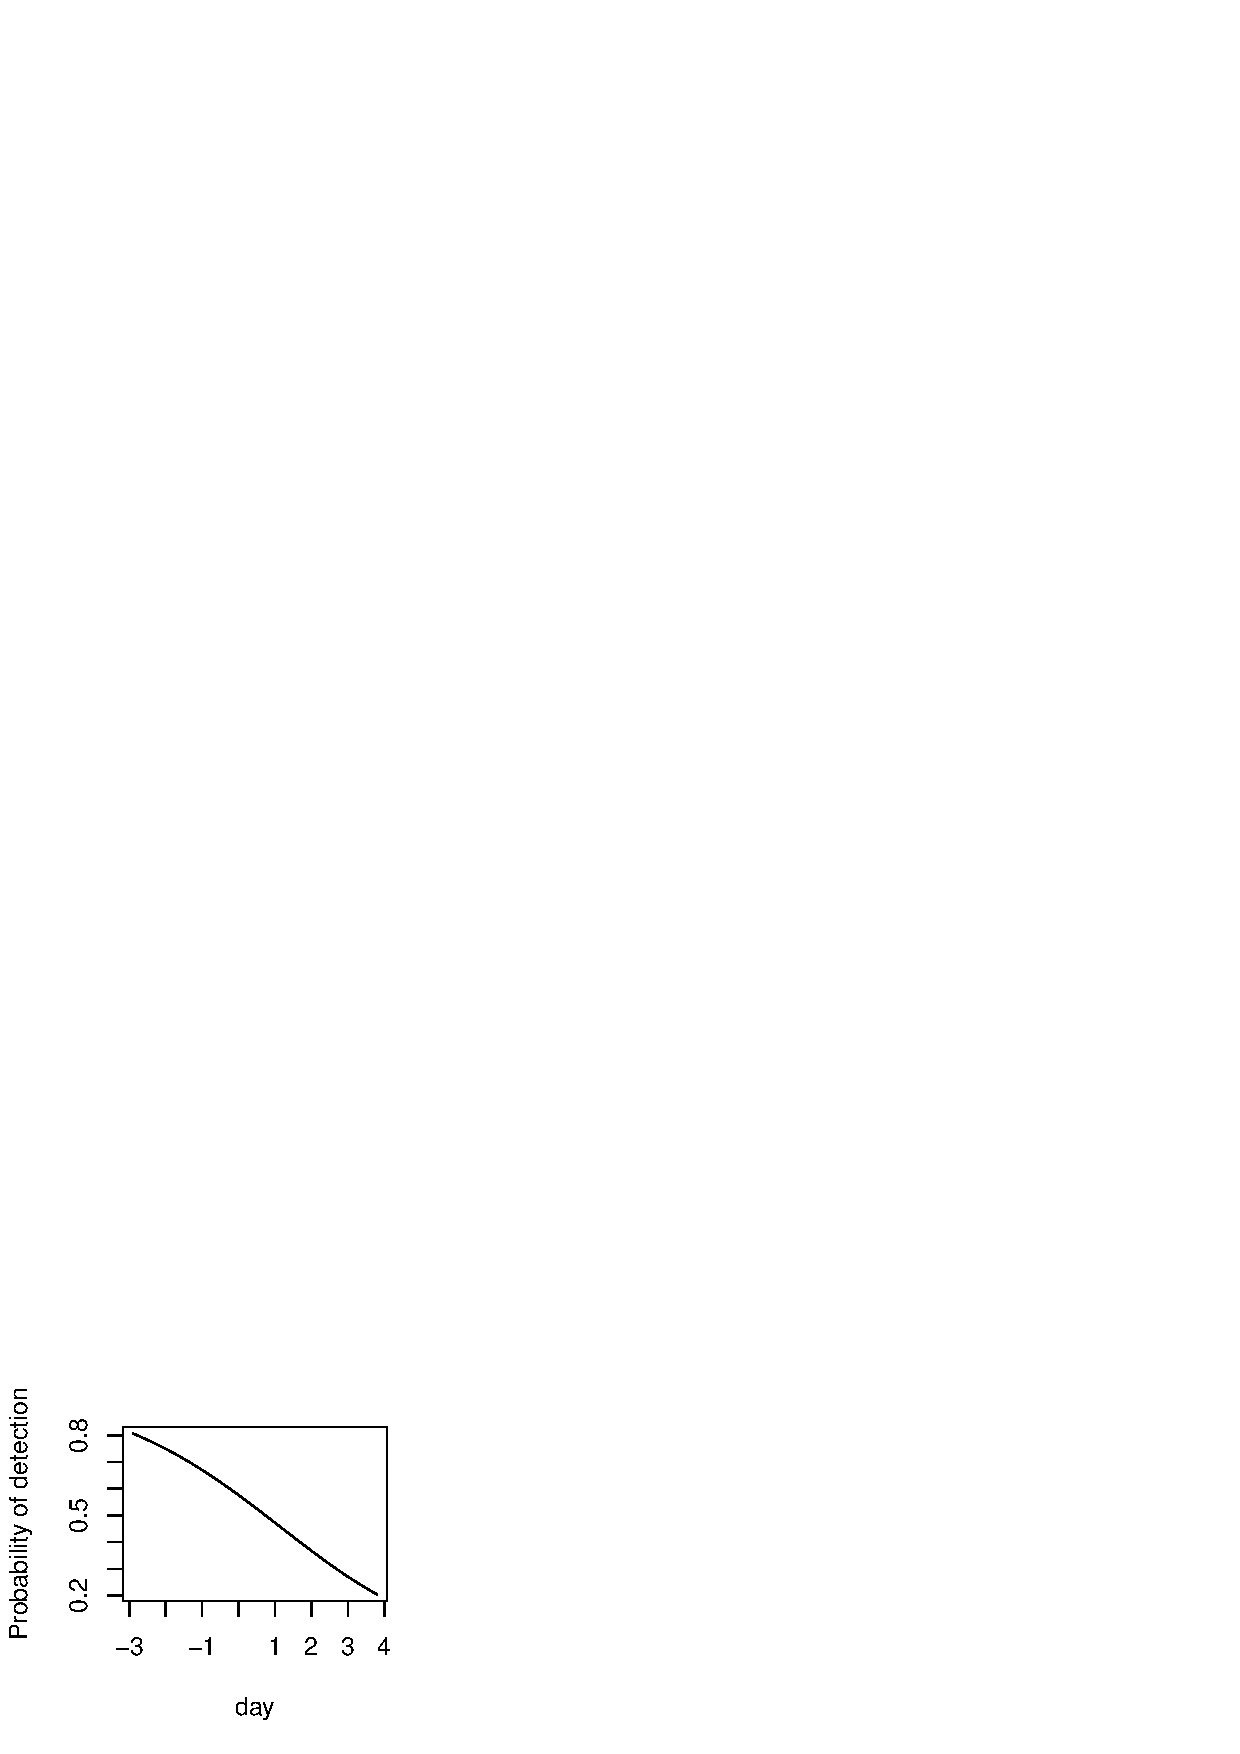
\includegraphics{unmarked-025}
\caption{Predicted detection probability as a function of day of year
  in the running mallard example}
\label{fig:preddet}
\end{figure}

\subsubsection{Parametric Bootstrap for Goodness-of-fit}

AIC can be used to select the best model in a set, but it does not indicate
how well a model fits the data.  
To conduct goodness-of-fit tests, \um\ provides a generic
parametric bootstrapping function.  It simulated data from the fitted
model and the computes summary information from any specified
statistic, with the default being the sum of squared residuals.


\begin{Schunk}
\begin{Sinput}
> set.seed(1234)
> (pb <- parboot(fm, statistic = SSE, nsim = 100))
> plot(pb, main = "Goodness-of-fit Parametric Bootstrap")
\end{Sinput}
\end{Schunk}

The above call to \code{plot} with a parametric bootstrap object as
the argument produces a useful graphic for assessing goodness of fit
(see Figure~\ref{fig:pb}).  The plot suggests that the model can adequately
explain these data.

\begin{figure}
  \centering
\begin{Schunk}
\begin{Soutput}
t0 = 463.4353 
152.1, 181.9
158.7, 124.6
146.4, 165
174.1, 135.1
161.1, 129.6
\end{Soutput}
\end{Schunk}
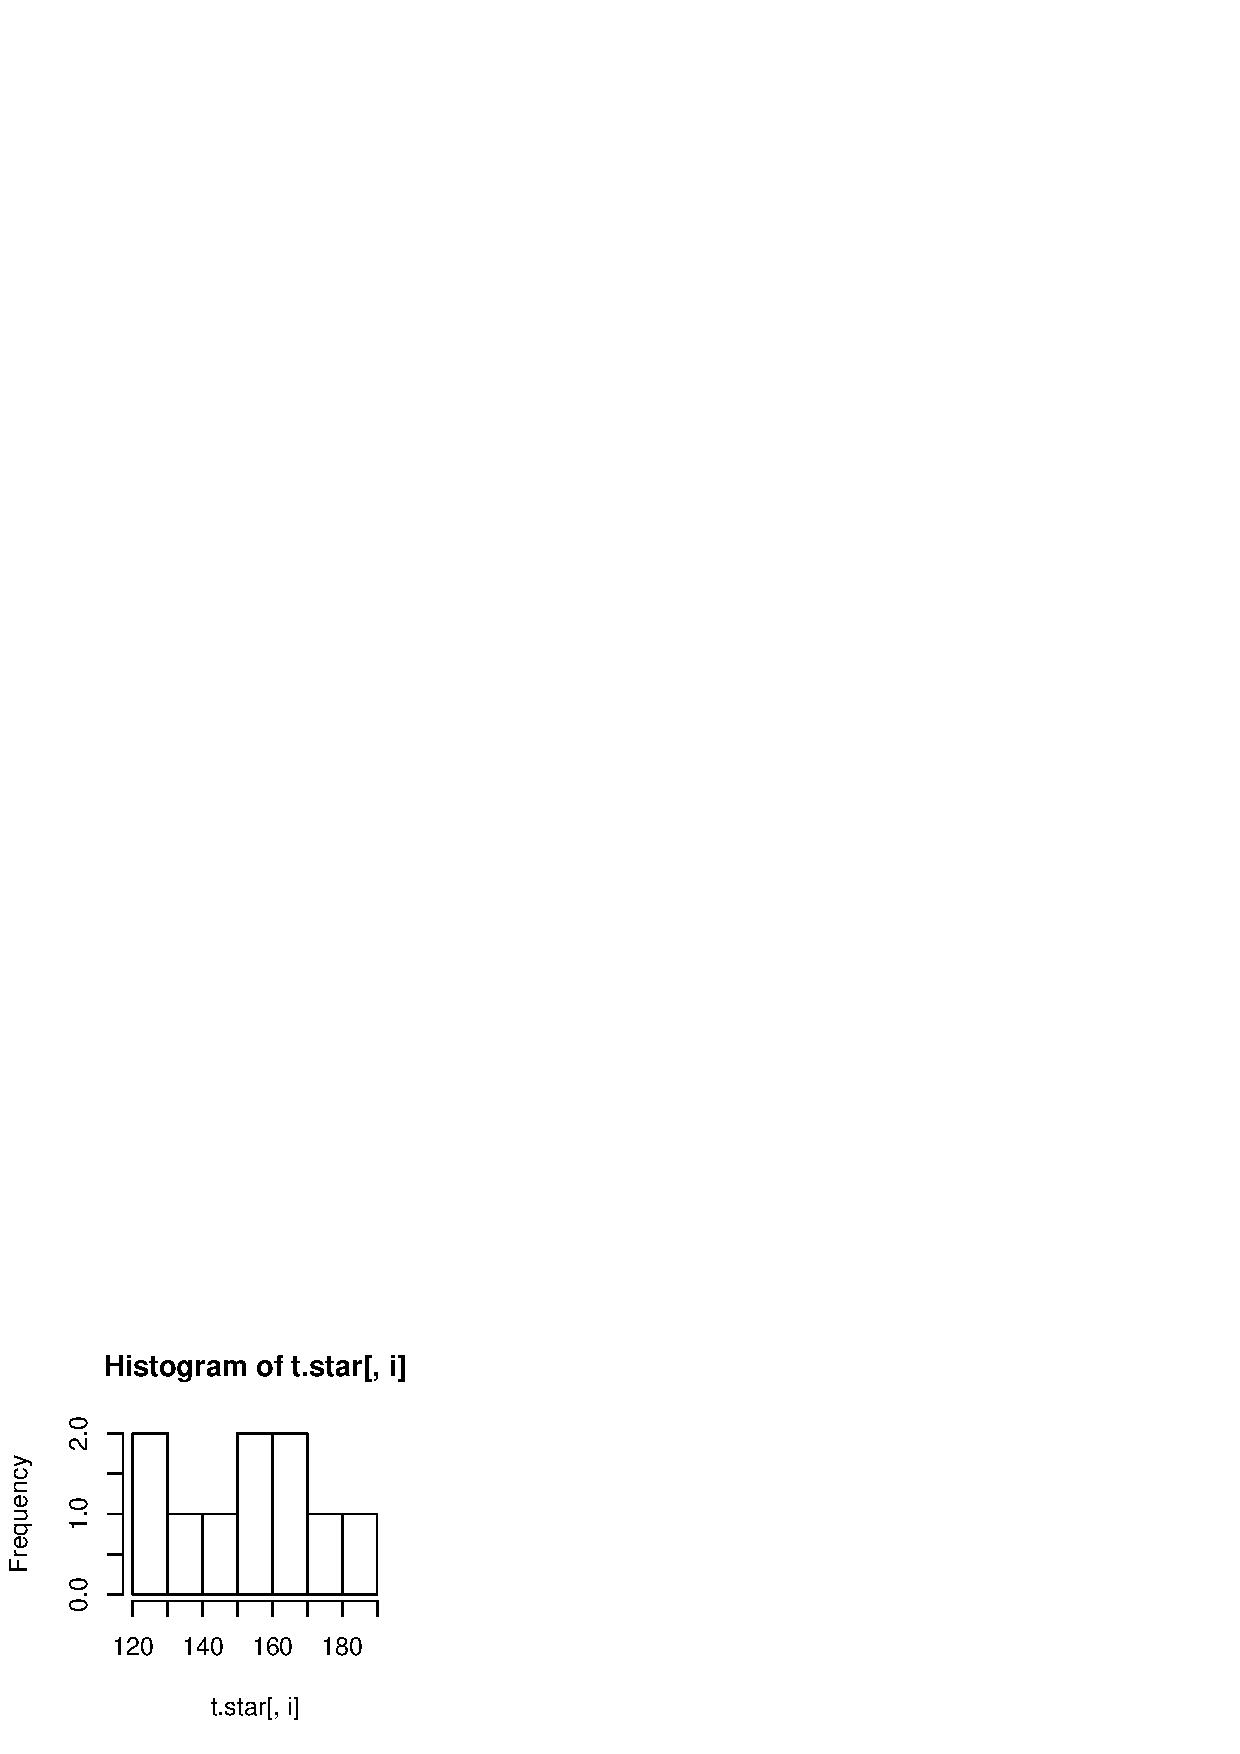
\includegraphics{unmarked-027}
\caption{Graphically assess model fit by parametric bootsrapping
  the sum of squared residuals.}
\label{fig:pb}
\end{figure}

\section[Future directions for unmarked development]{Future directions for \um\ development}
\label{sec:future-direct-unmark}

\um\ has become a stable and useful platform for the analysis of
ecological data, but 
several areas of development could improve its utility.
Bayesian estimation could be implemented for many
of these models.  This would provide a useful comparison with the
maximum likelihood results.  Random effects are an often requested
feature from users that will likely be incorporated into a future
version.  Random effects are useful for modeling heterogeneity among
sites that is not accounted for by covariates alone.  For maximum
likelihood methods, the Laplace approximation to the integrated
likelihood approach is likely to be fruitful and the incorporation of
random effects into Bayesian estimation is even more straightforward.

\um\ can be obtained from
CRAN within \rlang\ by issuing the command \\
\begin{Code}
install.packages("unmarked").
\end{Code}

% TODO: fix title case in bib file for titles.
%\bibliographystyle{jss}
\bibliography{/home/ian/Documents/bibtex/dissertation}

\end{document}
